\section{Final Assembly}

Upon the finalization of the optical design a conversion from laboratory bench design into a flight ready model. The transformation of the system will be discussed including the opto-mechanical design which would affix all the optical components to the main frame of ALI and baffle design and stray light reduction required for good SNR in ALI. Following the completion of ALI's system a brief overview of the control software used for the flight and testing the was underwent before launch.

\subsection{Opto-Mechanical Design}

After the telescopic system had been finalized for the optical chain a opto-mechanic case to hold the optical components needed to be design that would hold the competing in place during the flight and with stand the forces exserted upon during the launch of the stratospheric balloon and need to be satisfied for a twofold purpose. First, without suitable optical housing ALI's optical chain could become misaligned or damaged during the launch resulting in images either being of poor quality or completely out of focus. Second, in order to be able to mount ALI onto the stratospheric payload a the opto-mechanical case and design must be able to withstand certain safety values for torque and forces on the instrument during launch and flight to remove any debris from breaking off the gondolas to verify the safely of CNES workers who launch the balloon as well as citizens below the gondola during flight.

Consideration for thermal expansion and contraction of the opto-mechanical components also had to be considered when picking materials to house the optical lens housing system in order to reduce the chance of any torques arise in the optical chain from thermal expansions. To reduce this effect a consistent material was picked for the complete optical housing so all material would have the same thermal response to the environment it is exposed. Aluminum was the material chosen for the house since it is common used in stratospheric balloon instruments and platform because of its light weight and relatively inexpensive cost.

The next consideration was opto-mechanical housing design after a choice of material was style of the case. Commonly space based instrumentation uses a solid piece of material and is machined into a shape required to be able to house all the optical components. However, this method is relatively expensive and is generally used for finalized space instrumentation and not for design concept prototypes. These types of cases also have a long lead-time for the production and manufacturing component which would have been pressing our timeline for the launch date. The other option was to design an optical rail system primarily from preexisting components from known optical manufacturers, which would allow the flexibility to be able to make slight modifications to the design without having to commissioning a new one-piece case allowing for inexpensive alternation to the ALI optical chain without complete reconstruction. However, the draw back arise since with only using off-the-shelf components alignment and and resolution of the system may be harder to maintain. Considering the prototype nature of the project the choice was made to go with off-the-shelf opto-mechanical and structural pieces for ALI with the limitation in possible alignment and resolution being classified as an acceptable trade-off.

\begin{figure}[h!]
    \begin{center}
    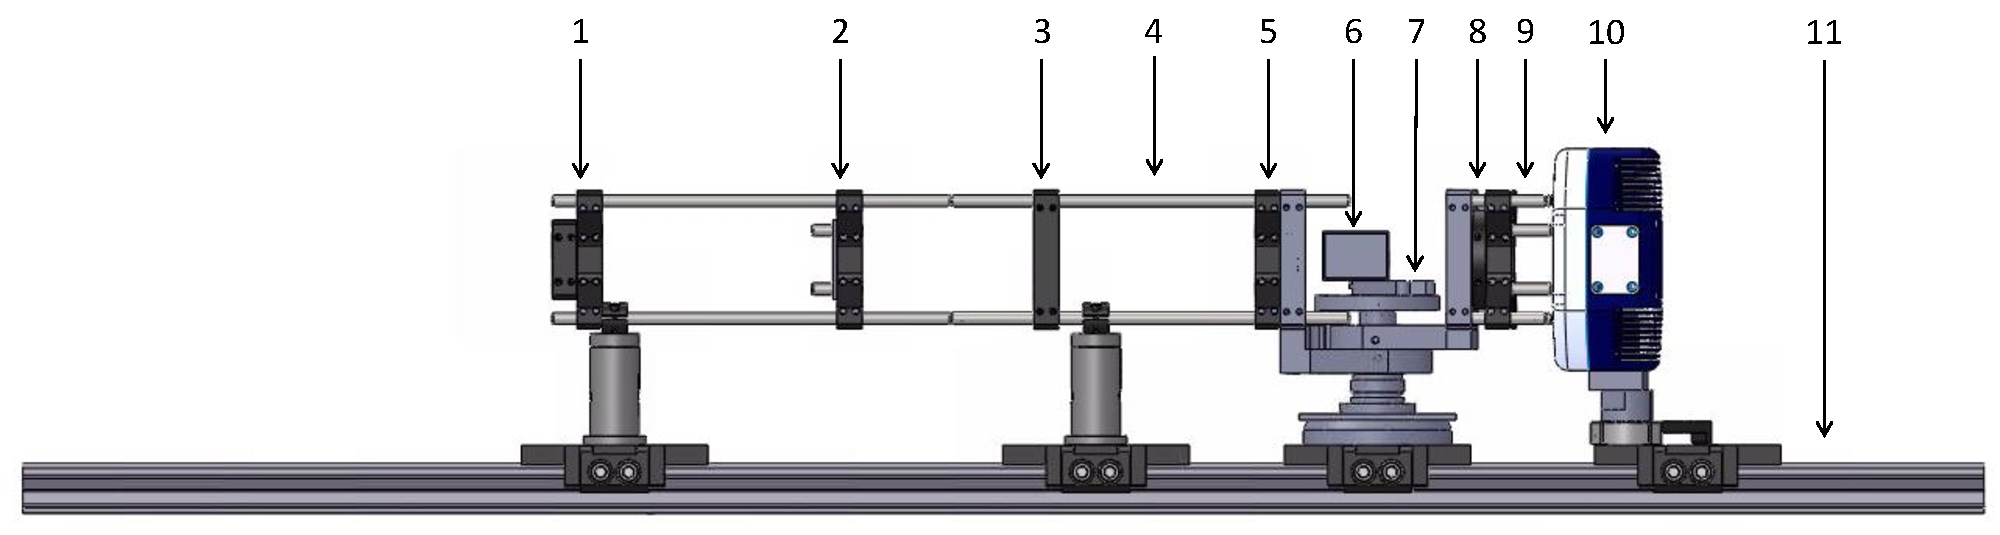
\includegraphics[width=1.0\textwidth]{./Images/3-3-OptoMechanicalSolidWorksLayoutProfile.pdf}
    \caption[ALI's Opto-mechanical Layout]{The final optical layout of ALI's optical chain from the profile perspective with the components being the following: (1) 150~mm plano-convex lens with 25.4~mm diameter. (2) Slit plate. (3) 100~mm plano-convex lens with 50.8~mm diameter. (4) Optical rail system. (5) Vertical linear polarizer. (6) Brimrose AOTF. (7) Rotation Stage. (8) Horizontal linear polarizer. (9) 50~mm bi-convex lens with 25.4~mm diameter. (10) QSI CCD camera. (11) Optical rail.}
   \label{fig:3.3:optoMechanicDesign}
    \end{center}
\end{figure}

Using components from ThorLabs, Edmund Optics, and McMaster-Carr an opto-mechanical case was design for the ALI instrument and can be seen in \autoref{fig:3.3:optoMechanicDesign} with noticed elements in the opto-mechanical system. A single sturdy wide optical rail, element 11, was used as the system base since it have the whole optical chain plus an undesigned baffle on it without have to concern about rail alignment and movement during flight. The large rail mount that the rail uses also allow for addition structure and support needed by the weight of the camera and the ability to align a future baffle with the optical chain. For the optical chain a system needed to be picked that would be rigid and keep the system in good alignment even under the stresses applied to the system during liftoff and flight. An optical cage was used, which can be noted as element 4, which allows each lens holder to be supported and held in place by all four corners of the optical cage and the lenses could be locked and glued into location.

During the testing of the optical system two prisms were used account for the bend in the optical chain caused the AOTF which needs to be removed from the final system due to distortions caused by the prisms within the system. A rotation stage was added with the pivot point being the AOTF compensating for the 2.7\si{\degree} optical axis bend.

The optical components were purchases to the the specification required from the design with a few addition modifications. First, the lenses were ordered with an antireflection coating in order to increase the systems efficacy, a B-type antireflection coating was order for the lenses from ThorLabd with reduces reflection from the lens surface down to an average of less than 0.50\% from 650 to 1050~nm instead of an 8\% loss per surface from an uncoated lenses. The lenses also had a tolerance of a a 1\% error in the focal length and made form grade A N-BK7 glass. The linear polarizer used, elements 5 and 8, were purchased and a selection of linear polarizer were considered. However the wavelength range of ALI made standard polarizer difficult to find which limited the possible choices. A nanoparticle linear film polarizers was eventually decided upon even though it was one of the more expensive polarizer options but gave an extinction ratio of since it was greater than 100,000:1 for 650 to 1200~nm completely covering ALI operating range. The extinction ratio is defined by the ratio between the maximum transmission when the polarizers axis is aligned with the signal to the minimum transmission after the polarizer has been rotated by 90\si{\degree}.

\begin{figure}[h!]
        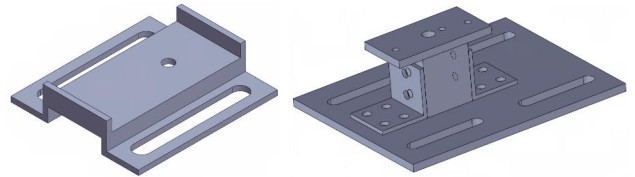
\includegraphics[width=\textwidth]{./Images/3-3-CustomMountingPieces.pdf}
        \caption[ALI Custom Mounting Hardware]{The custom mounting hardware design to mount the AOTF and QSI CCD camera into ALI's opto-mechanical design. Left: Custom AOTF mounting hardware. Right: The five piece QSI CCD camera mounting hardware.}
        \label{fig:3.3:aotfCustomMount}
\end{figure}

Lastly, consideration had to be given to mounting the AOTF and CCD camera. Both of these elements are are non-standard sizes in optics and no preexisting components could be purchased to mount these pieces. Custom mounting pieces were used designed both components and were design though solid works. The AOTF had one usable mounting hold on the bottom of the device to affix the device to the optical chain. However, directly mounting the device onto the rotation stage would result in the AOTF being offset downward from the optical path. Furthermore with only one mounting point there was concern for rotation of the device during the flight. A piece was designed that lightly clamped the AOTF onto the top of the mounting hardware to lock the AOTF's rotation axis and then use the four slot screw holes located on the lower plane to center the device into the center of the rotation stage which can be seen in the left side of \autoref{fig:3.3:aotfCustomMount}.
 
The mount for the CCD camera had a different set of requirements, mounting holes were available for use on the bottom of the camera but the camera mount needed to be able to securely hold the relatively heavy camera into place with very little space was available between the base of the rail mount and the camera for the design. A five piece mount was designed that would fit in the tight space and be study to support the mass of the camera seen in the right side of (\autoref{fig:3.3:aotfCustomMount}. The base plate perfectly fits onto the optical rail mount and the slotted holes allows for horizontal alignment of the camera with the optical axis with the vertical alignment being correctly set with the mount height. Also the CCD sensor on the QSI camera is offset to one side so to account for the offset the mounting hardware for the camera is offset from the center.


\subsection{Baffle Design}

A BASIC START:

Many questions arose when the baffle for the ALI system was devised. Questions arose over length and width of the baffle as well as how many baffles should located in the final design as well as the interior shape of the baffle layout. These were all important questions that needed ansering since stray light rejection from the ALI insturment is crutial in order to achieve high sensitivity of the light from the atmoshere.

The baffel system is designed such that all light entering the system hit at least 3 surfaces before it can enter the opical system for direct scattering and 2 surfaces for indirect scattering. This methoid is called the thriple bounce disign and i standeredly used in opticals to minimise stray light. In the system the baffels are spaced in such that no stray light that can enter the system is minimized by having the stray light hit three incoming surfaces reducing the overall intersity of the light.

The first point of the discussion was a hight versus width discussion. IN a baffle system the larger the baffle is by shear volume the better the baffle can be designed to reduce stray light. However there is a limited amount of space to build the ALI instrument and the baffle must share space with optics, eletronics and power systems; as such a size had to be selected. A height and width of 70 mm was choosen. The CCD camera used in the design had a height of a little greater then 70 mm and did not want the instrument to have to be any taller. This left the length of the baffle to be determined. The length is also limited by the space for ALI as well as the field of view and entrance apperture size, and its location. One always needs to make sure the the optical stop is the location that limits the amount of light that is entering the system. If this is artifically changed with the baffle design it will affect the preformance of the instrument itself. If the optical stop is moves further from the optical system one keeps the same field of view but limits the amount of light that enters the system. Thus changing the overall F/\# of the system and either increases the exposure times or decreases the signal to noise ratio. The other case is if the optical stop is moved closer to the optical system, which causes the opposite problem which is more light enters the system than the system was designed for causing an excess of stray light and rendering the baffel useless.

This information leaves us with three kinds of fundimental locations to put the optical stop of the system in the design phase. The first is to put the optical stop as close ot the front lens as possible, second is to place the optical stop at the far end of the baffel, and third to place the optical stop in the middle of the baffle system. IN the first case the baffels have a  diverging shape and there are few baffles. In the second case

Although the overall choice between these three do not have  a great effect on the effencey of the baffle itself it has an effect on the shape on the baffle system as well as the number of baffles required. The greatest difference is the change in the optical system required, the further away the optical stop is from the front lens the larger the optical components need to be in order to accept all of the light, which makes the system heavier, larger and more expensive to build. In ALI the optical the stop was choosen to be close to the first lens to make the system has small and compact as possible as well has to reduce the number of baffels that needed to be built for the system and thus the overall cost with reducing the systems effectivness.

\subsection{Control Software}

\subsection{System Testing}
